\documentclass{llncs}
\setcounter{tocdepth}{5}

\setcounter{secnumdepth}{5}
\usepackage{xcolor}
\usepackage{graphicx}
\usepackage{listings}
\usepackage[utf8]{inputenc}
\lstset{language=Verilog,breaklines=true,basicstyle=\footnotesize, frame=single}
\usepackage{scrextend}
\usepackage{hyperref}
\hypersetup{
    colorlinks,
    citecolor=black,
    filecolor=black,
    linkcolor=violet,
    urlcolor=black
}

\usepackage{pdfpages} 

\begin{document}
\raggedbottom

\title{MIPS in Verilog}
\author{Nathan St. Amour \& Colt Kiser}
\institute{Ohio University, Athens, OH 45701}

\maketitle

\begin{abstract}
  This report describes an implementation of a subset of the MIPS instruction architecture as described in class and the book\cite{1}.
  The implementation is simulated using the architecture modeling language Verilog. Included in our implementation is a language of instructions
  that is broken down into three types: The memory-reference instructions(lw and sw), the arithmetic logic instructions(add, sub, AND, OR,
  , and branch instructions(j and beq).  These instructions can be used to implement
  a simple language.  It includes several fully functional logic units that are brought together to define the semantics of each instruction
  on simulated hardware. We will describe the modules used to realize this design and the methodology that allows MIPS be a successfull
  implementation and any problems that have arisen while implementing the processor. 
\end{abstract}

\begin{addmargin}[-5em]{-2em}
  \cite{1}
  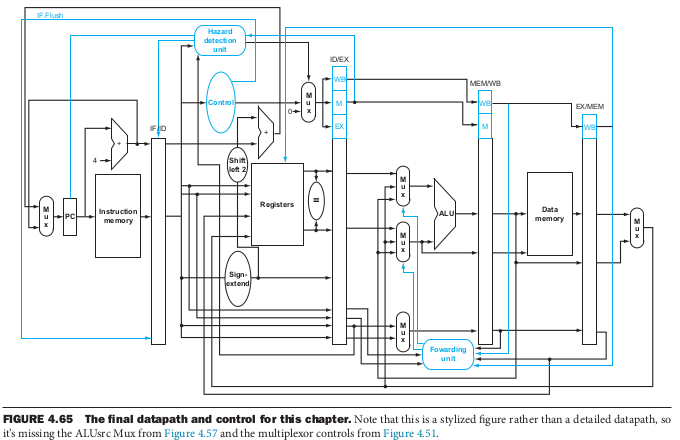
\includegraphics[scale=.6]{mips.png}
\end{addmargin}

\tableofcontents  
\newpage
%% \begin{addmargin}[-4em]{-4em}
%%   \begin{lstlisting}
%%     output [2:0] ALUControl; // 3-bit output for controlling ALU based on ALUOp and function code
%%   \end{lstlisting}
%% \end{addmargin}

\section{Introduction and MIPS Design}


\subsection{MIPS}
MIPS. is a reduced instruction set(RISC),  Our implementation is going to be pipelined vs multicycle.  It can be used for embedded devices,
microcontrollers or for a wide range of other styles of computing.  MIPS is used in embedded systems such as: windows ce devices, gateways and some video game implementations.

\section{Design Methodology}
The MIPS instruction set is designed with the ideal of a simple instruction set that includes instructions that largely use the same set of
 logical operations to carry out their task.  Our design methodology stays true to that, especially with the small instruction set.  We implement
 all of the basic features of a MIPS processor.  This design includes an Instruction memory, Registers, Data memory, ALU operations etc...
 We also looked into implementing Forwarding(\ref{f:1}) to solve harzards but did not have enought time to get it to work properly with the final MIPS design. 
 \subsection{Mips Data Storage}
 We have split up the Instuction memory and Data memory in order to prevent to the hazard that would result from trying to fetch
 an instruction and read or write to the Data memory at the same time.  So the memory that stores instructions ends up being separated from the main Data memory.  There is also a register file which allows for functionality of registers. Registers provide quick lookup to data for operations.  This allows the slow main memory to be used for writing and lookup less frequently.  The Data memory include 128 words for long term storage of data.  This Data memory is used by instructions sw and lw.

 The Data memory module is described in greater detail in the section further into the document \ref{eq:1}

 The Instruction memory stores the value of the PC counter and the different types of instructions that we have implemented in our MIPS implementation.  \ref{inst:1} \cite{1}
\section{Instruction Set}
  The MIPS instruction set includes three types of commands:  R-type, I-type, J-type. All three of the command types share
  have some regularities.  This allows for the use of a reduced number of features in hardware to implement the instructions.  \cite{1}


\section{Processor Purpose/Functions}
  The processor can be used to do anything that can be imagined by the small set of instruction and state which are implemented in the code corresponding with this report.  The 5 stages of our pipelined MIPS processor are implemented here: IF, ID, EX, MEM, WB.  The processor could be further extended to allow for forwarding and other hazard mitigation techniques.  The beq instruction does not work without forwarding so without that functionality we cannot use the branch equal command.
  
\subsection{Modules}
The module system in Verilog provides an essential feature of abstraction.  A module is written to perform a specific task that may include several instructions which is then used to implement more general features by passing inputs and outputs to the module and using the affected outputs.
\subsubsection{MIPS}
This is our attempt at bring together all of the modules and stages in order to have a fully functional processor.  We have implemented three instructions with opcode shown in the test bench. \ref{mips:1}  We learned a lot during this stage but failed to completely tie together all of the peices into a fully functional processor.  
\subsubsection{IF}
The IF module that we implemented will take care of the Instruction Fetch stage of the MIPS instruction pipeline. The purpose of the module is to fetch the instruction opcode, which identifies the instruction is being executed, from the instruction memory. The other responsibility of the IF module is to increment the Program Counter (PC) each time an instruction is executed. Our implementation increments the counter by a value of 1 each time an instruction is implemented.\ref{if:1}

\subsubsection{ID}
The purpose of the ID module is to complete the Instruction Decode stage of the MIPS instruction pipeline. The main purpose of this stage of the pipeline is to simply figure out what the instruction returned by the IF stage of the pipeline is supposed to do. The ID module figures out what the instruction is from the opcode and breaks apart the instruction code into its different parts. This step also decides what registers are required and can make this decision before the instruction is fully decoded due to the simple instruction format it is given. \ref{id:1}
\subsubsection{EX}
The main purpose of the EX module to do the calculations that are required for the connection. This includes doing the arithmetic calculations required in mathematical instruction, like add or sub, and calculating memory references or adding up base and offset values. Our implementation uses a 32bit ALU that we created to calculate these values. 

\subsubsection{MEM}
The MEM module in our project handles all the memory access required for MIPS commands. This module is used if an instruction needs to load, store, or access data that is stored in memory. This stage of the pipeline also replaces the PC with a destination address if the instruction a branching instruction. If the instruction does not require either of these functions, then this module does nothing.\ref{mem:1}

\subsubsection{WB}
The purpose of the WB module is to handle the Write Back part of the MIPS pipeline. This module has one simple function. This is to place the results of the instruction in the appropriate register, which is designated in the instruction. \ref{wb:1}

\subsubsection{Data memory}
The DataMemory module that we implemented either reads or writes and address from a specific register in memory. You can find the data memory here: \ref{eq:1} 

\subsubsection{Instruction Memory}
This is the Instruction memory.  All commands use the instructions
memory and the PC counter uses it as well.

In our module for the Instruction memory takes as input an instruction
address and an instruction to be returned (instruction\_address,
instruction). The instruction address is declared as a 32bit input and
the instruction is a 32bit output. The instructions are then loaded
into the 32bit register file instruction\_memory\_file.  Then as
needed the instruction memory register, instruction\_memory\_file is
used to lookup the correct instruction address.  Find the code to the
instruction memory in the appendex. \ref{inst:1}
 
\subsubsection{ALU}
The arithmetic logic unit of our MIPS implementation is used by all commands that we have implemented except for the jump command.  The ALU is 32 bit to correspond with the standard data size of a word that the MIPS design uses. The ALU is made up of many sub modules that are extracted away to make the logic of the Verilog implementation only 2 lines long.  The ALU takes 7 reasonable parameters as input.
\begin{description}
\item[1. a, b: ] The two 32 bit binary numbers (a,b) that are declared as 32 bit inputs in the Verilog
\item[2. op: ] The op-code that is declared as a 3 bit input
\item[3. result: ] The 32 bit output of the operation 
\item[4. set: ] The one bit output result of the most-significant ADDER unit
\item[5. zero: ] The one bit output that is set if the result is 0x00000000
\item[6. overflow: ] One bit output that is 1 if the output of an operation creates an overflow
\end{description}

The 32 bit then makes two calls to 16 bit ALUs with some temporary wires to help us with the structure of the Verilog. The ALU is referenced in the appendex here: \ref{alu:1}
\paragraph{16 Bit ALU}
The 16 bit ALU behaves in a similar way to the 32 bit version.  However it does make use of the CLA unit, described in \ref{cla:s}, and makes use of four 4 bit ALUs, the output of which is likewise combined into one 16 bit half word.  The 16 bit ALU is referenced here: \ref{alu:2}
\paragraph{4 Bit ALU}
The four bit adder uses a carry the Carry lookhead adder unit, \ref{cla:s} as well and makes use of four 1 bit ALUs. 
The 4 bit ALU that is implemented here: \ref{alu3} 
\label{cla:s}
\subsubsection{CLA}
The carry look ahead adder module uses the logic that was described in class and in the book to implement a 4 bit adder.  The logic behind it makes use of quickly predicting which bits will preform a carry.  You can find the CLA code here: \ref{cla:1}
\subsubsection{1 Bit ALU}
The one bit ALU is implemented per the design given to us on homework three.
\begin{center}
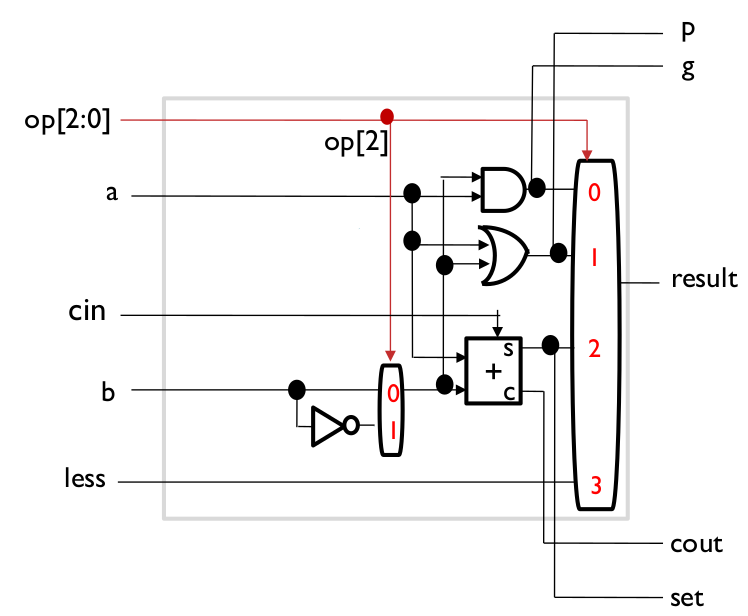
\includegraphics[scale=.4]{images/onebitalu.png}
\end{center}

\section{Conclusion}
We were able to successfully implement and test all five stages if the MIPS instruction pipeline successfully, however, the MIPS processor that we implemented does not work completely right. We created test benches for the five stages of the pipeline and we are convinced that they are working correctly. The test benches and waveforms created from the modules are included in the appendix of the report. Given more time to work on the project we are both confident that we could get together an implementation that had a fully functional set of commands.

\section{Appendex}
\subsection{MIPS}
\label{mips:1}
\begin{addmargin}[-5em]{-2em}
\lstinputlisting{../MIPSProcessor.v}
\end{addmargin}
\subsubsection{TB/WF}
\begin{addmargin}[-5em]{-2em}
  \lstinputlisting{../tests/MIPSProcessor_tb.v}
\end{addmargin}
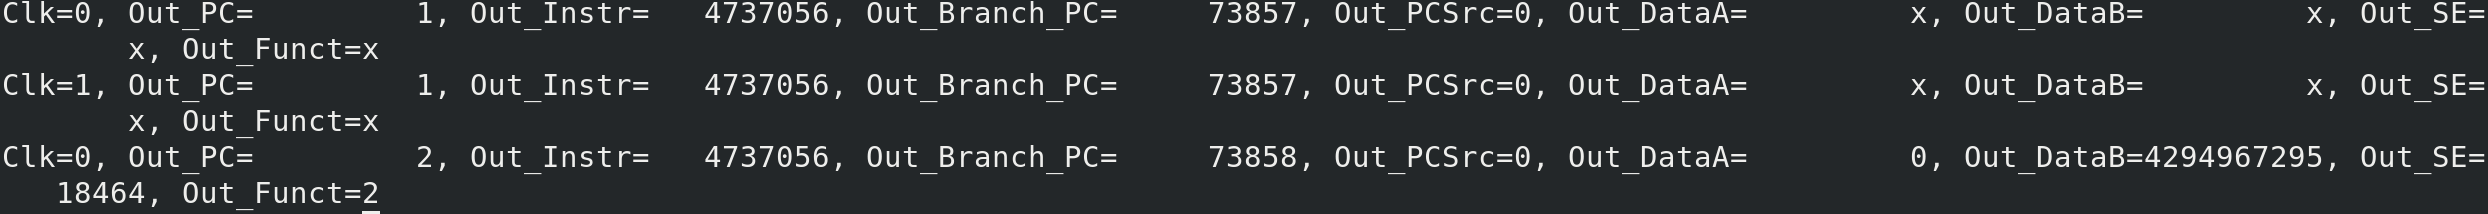
\includegraphics[scale=.2]{images/mipstb.png}



 % Done
\begin{addmargin}[-5em]{-2em}
\subsection{IF}
\label{if:1}
\begin{flushleft}
  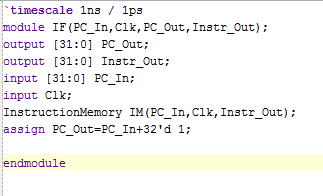
\includegraphics[scale=.6]{../Screenshots/IF.PNG}
\end{flushleft}
\subsubsection{WF/TB}
\begin{flushleft}
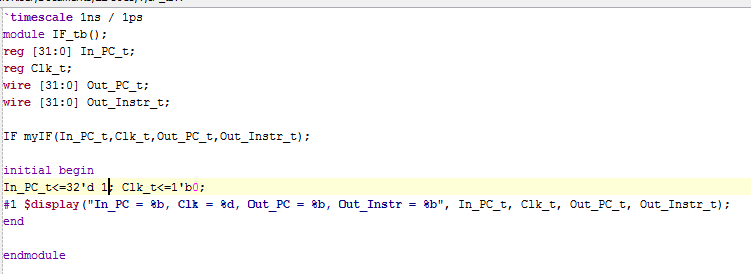
\includegraphics[scale=.6]{../Screenshots/IF_tb.PNG}
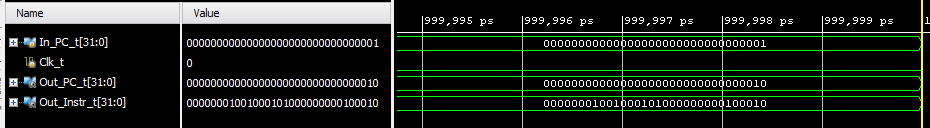
\includegraphics[scale=.6]{../Screenshots/IF_Waveform.PNG}
\end{flushleft}

\subsection{ID}
\label{id:1}
\begin{flushleft}
  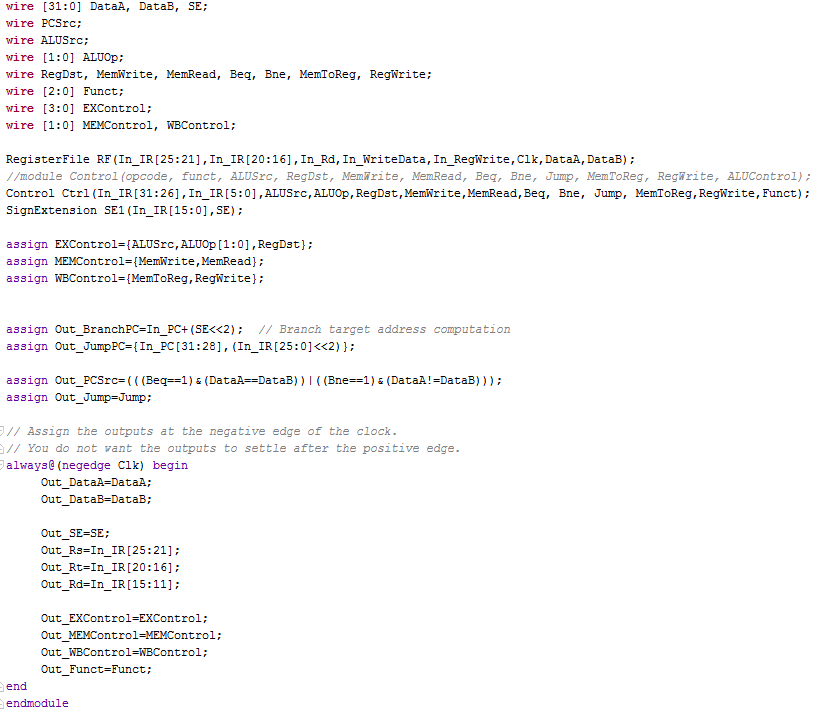
\includegraphics[scale=.6]{../Screenshots/ID.PNG}
\end{flushleft}
\subsubsection{WF/TB}
\begin{flushleft}
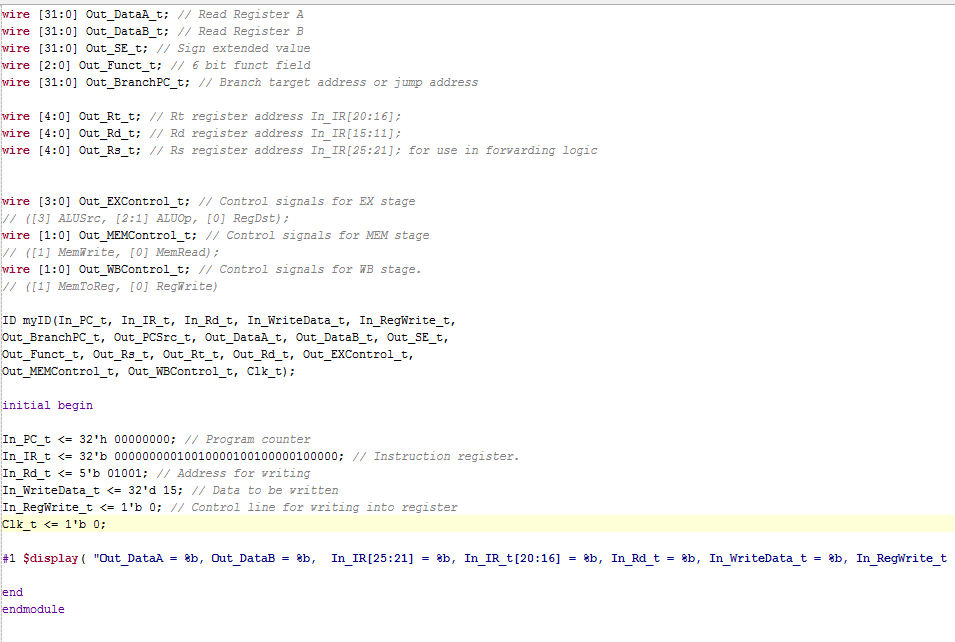
\includegraphics[scale=.6]{../Screenshots/ID_tb.PNG}
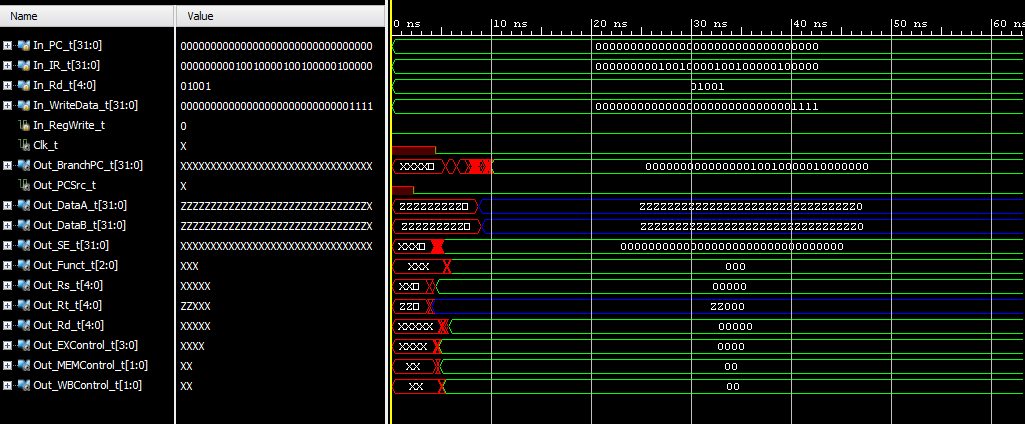
\includegraphics[scale=.6]{../Screenshots/ID_Waveform.PNG}
\end{flushleft}

\subsection{EX}
\label{ex:1}
\begin{flushleft}
  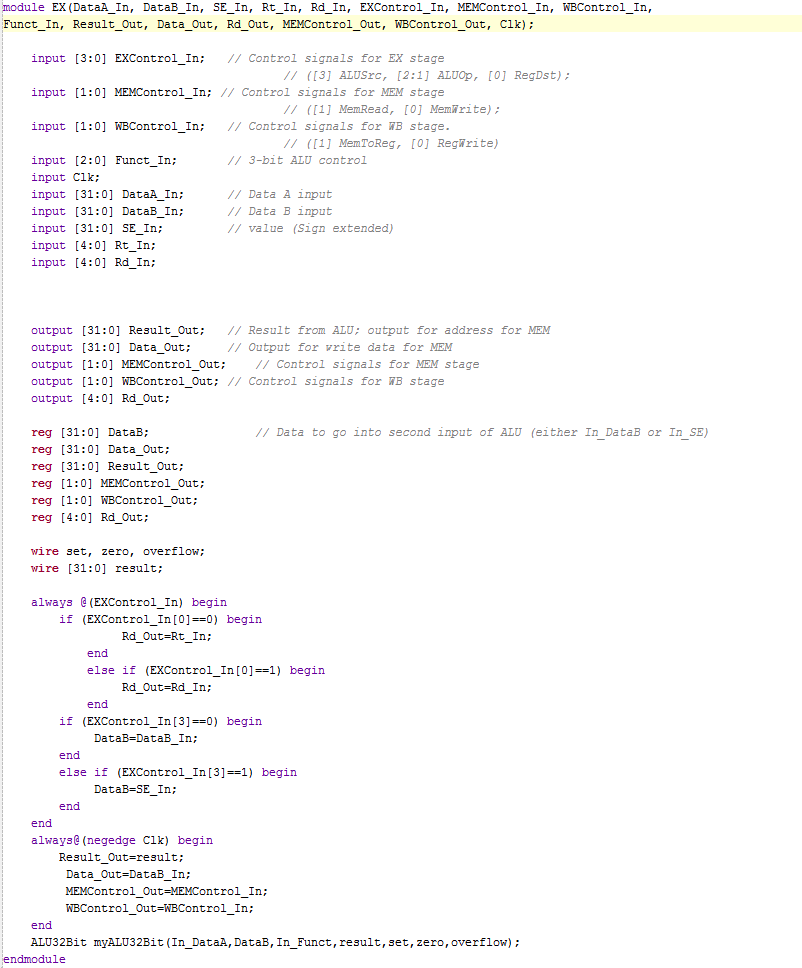
\includegraphics[scale=.6]{../Screenshots/EX.PNG}
\end{flushleft}
\subsubsection{TB/WF}
\begin{flushleft}
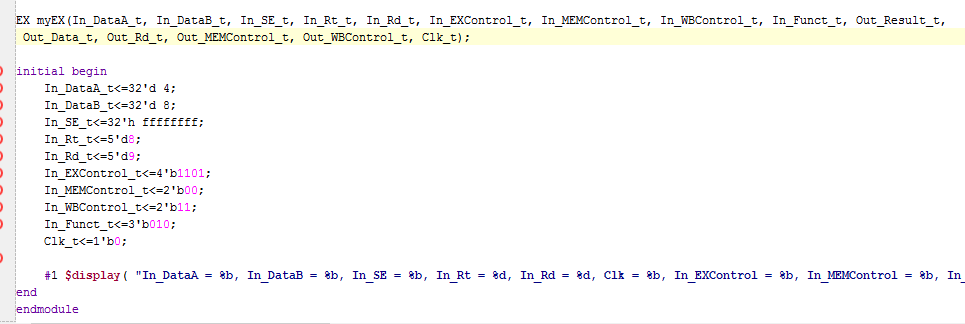
\includegraphics[scale=.6]{../Screenshots/EX_tb.PNG}
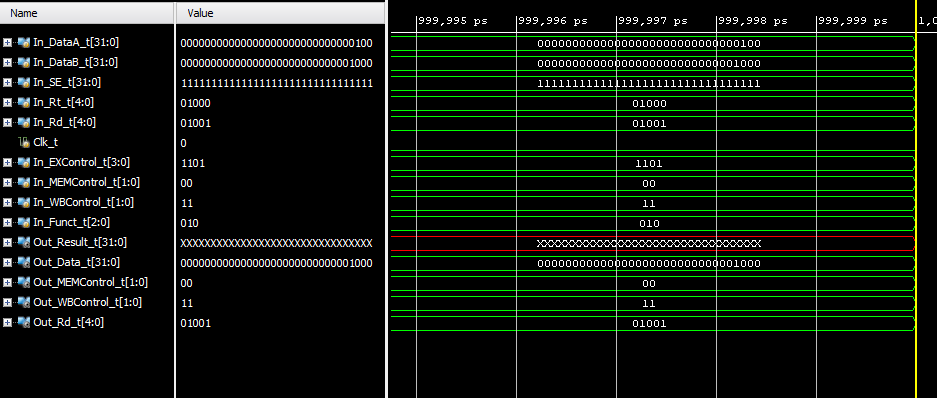
\includegraphics[scale=.6]{../Screenshots/EX_Waveform.PNG}
\end{flushleft}

\subsection{MEM}
\label{mem:1}
\begin{flushleft}
  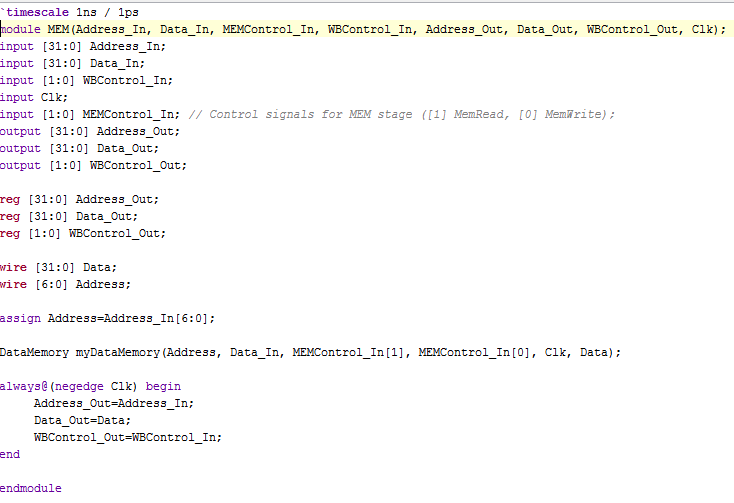
\includegraphics[scale=.6]{../Screenshots/MEM.PNG}
  \end{flushleft}
\subsubsection{WF/TB}
\begin{flushleft}
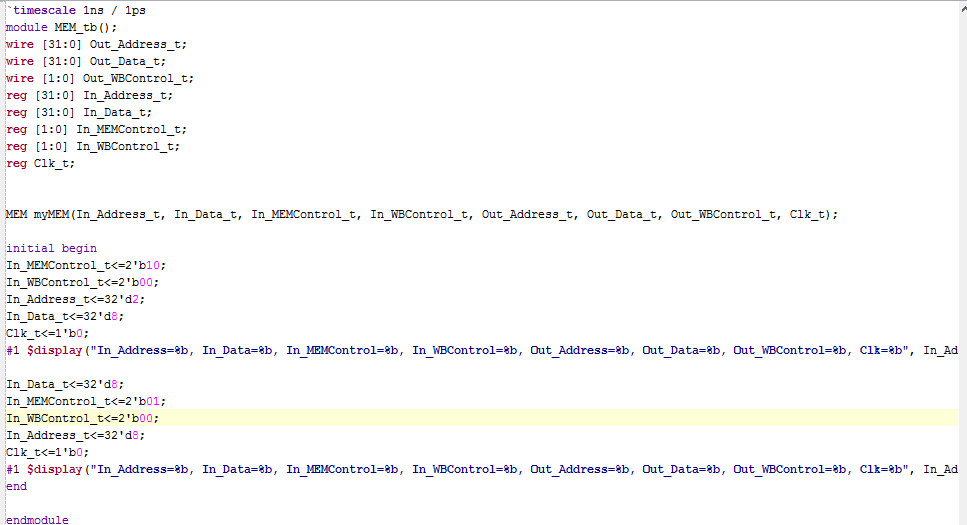
\includegraphics[scale=.6]{../Screenshots/MEM_tb.PNG}
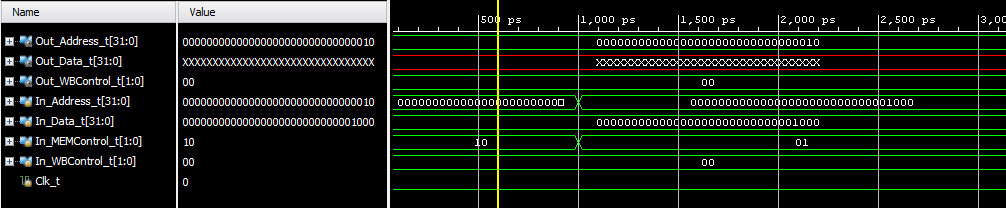
\includegraphics[scale=.6]{../Screenshots/MEM_Waveform.PNG}
\end{flushleft}

\subsection{WB}
\label{wb:1}
\begin{flushleft}
  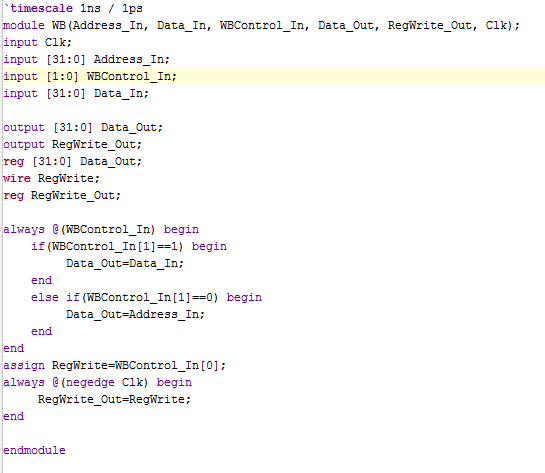
\includegraphics[scale=.6]{../Screenshots/WB.PNG}
  \end{flushleft}
\subsubsection{WF/TB}
\begin{flushleft}
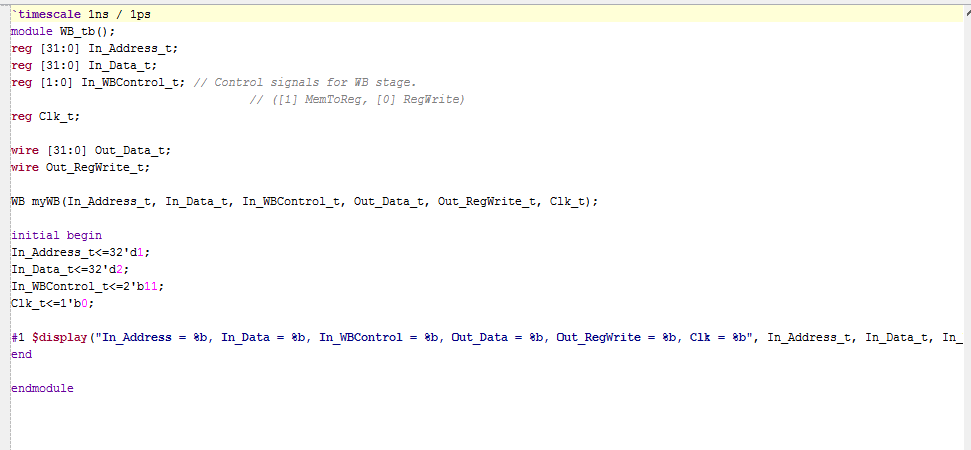
\includegraphics[scale=.6]{../Screenshots/WB_tb.PNG}
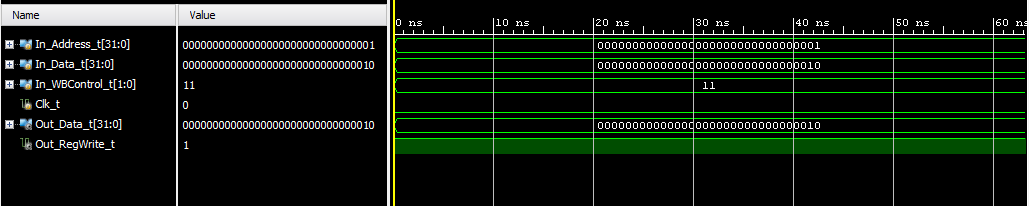
\includegraphics[scale=.6]{../Screenshots/WB_Waveform.PNG}
\end{flushleft}


\end{addmargin}


\subsection{Data Memory}
\label{eq:1}
\begin{addmargin}[-5em]{-2em}
\lstinputlisting{../dataMemory.v}
\end{addmargin}
\subsubsection{TB/WF}
\begin{addmargin}[-5em]{-2em}
  \lstinputlisting{../tests/DataMemory_tb.v}
\end{addmargin}
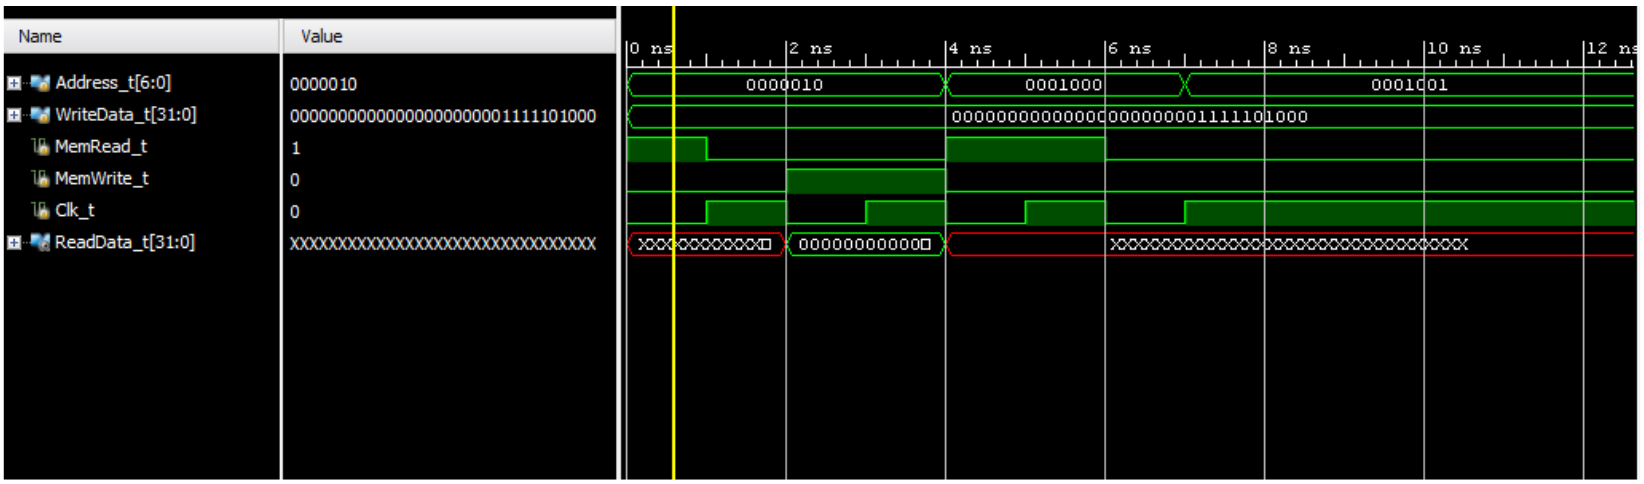
\includegraphics[scale=.2]{images/datamemory.png}



 % Done
\subsection{Instruction Memory}
\label{inst:1}
\begin{addmargin}[-5em]{-6em}
  \lstinputlisting{../InstructionMemory.v}
\end{addmargin}
\subsubsection{ TB/WF}
\begin{addmargin}[-5em]{-6em}
  \lstinputlisting{../InstructionMemory.v}
\end{addmargin}
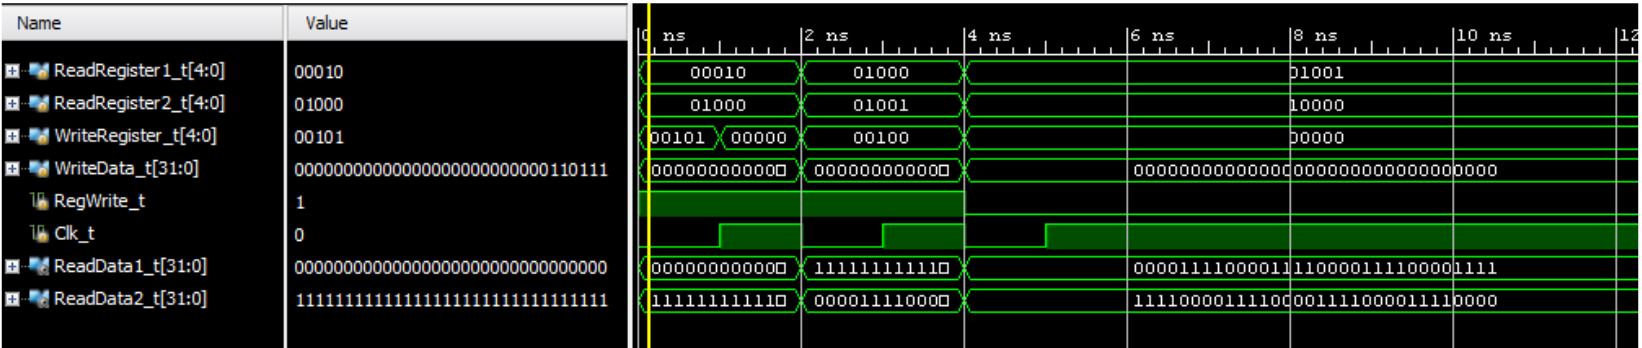
\includegraphics[scale=.2]{images/instmemory.png}
% Done
\subsection{Control}%Add description
\label{c:1}
\begin{addmargin}[-5em]{-6em}
  \lstinputlisting{../control.v}
\end{addmargin}
\subsubsection{TB/WF}
\includepdf[pages={8}]{../Homework5.pdf}


\subsection{Control Old} %same
\label{co:1}
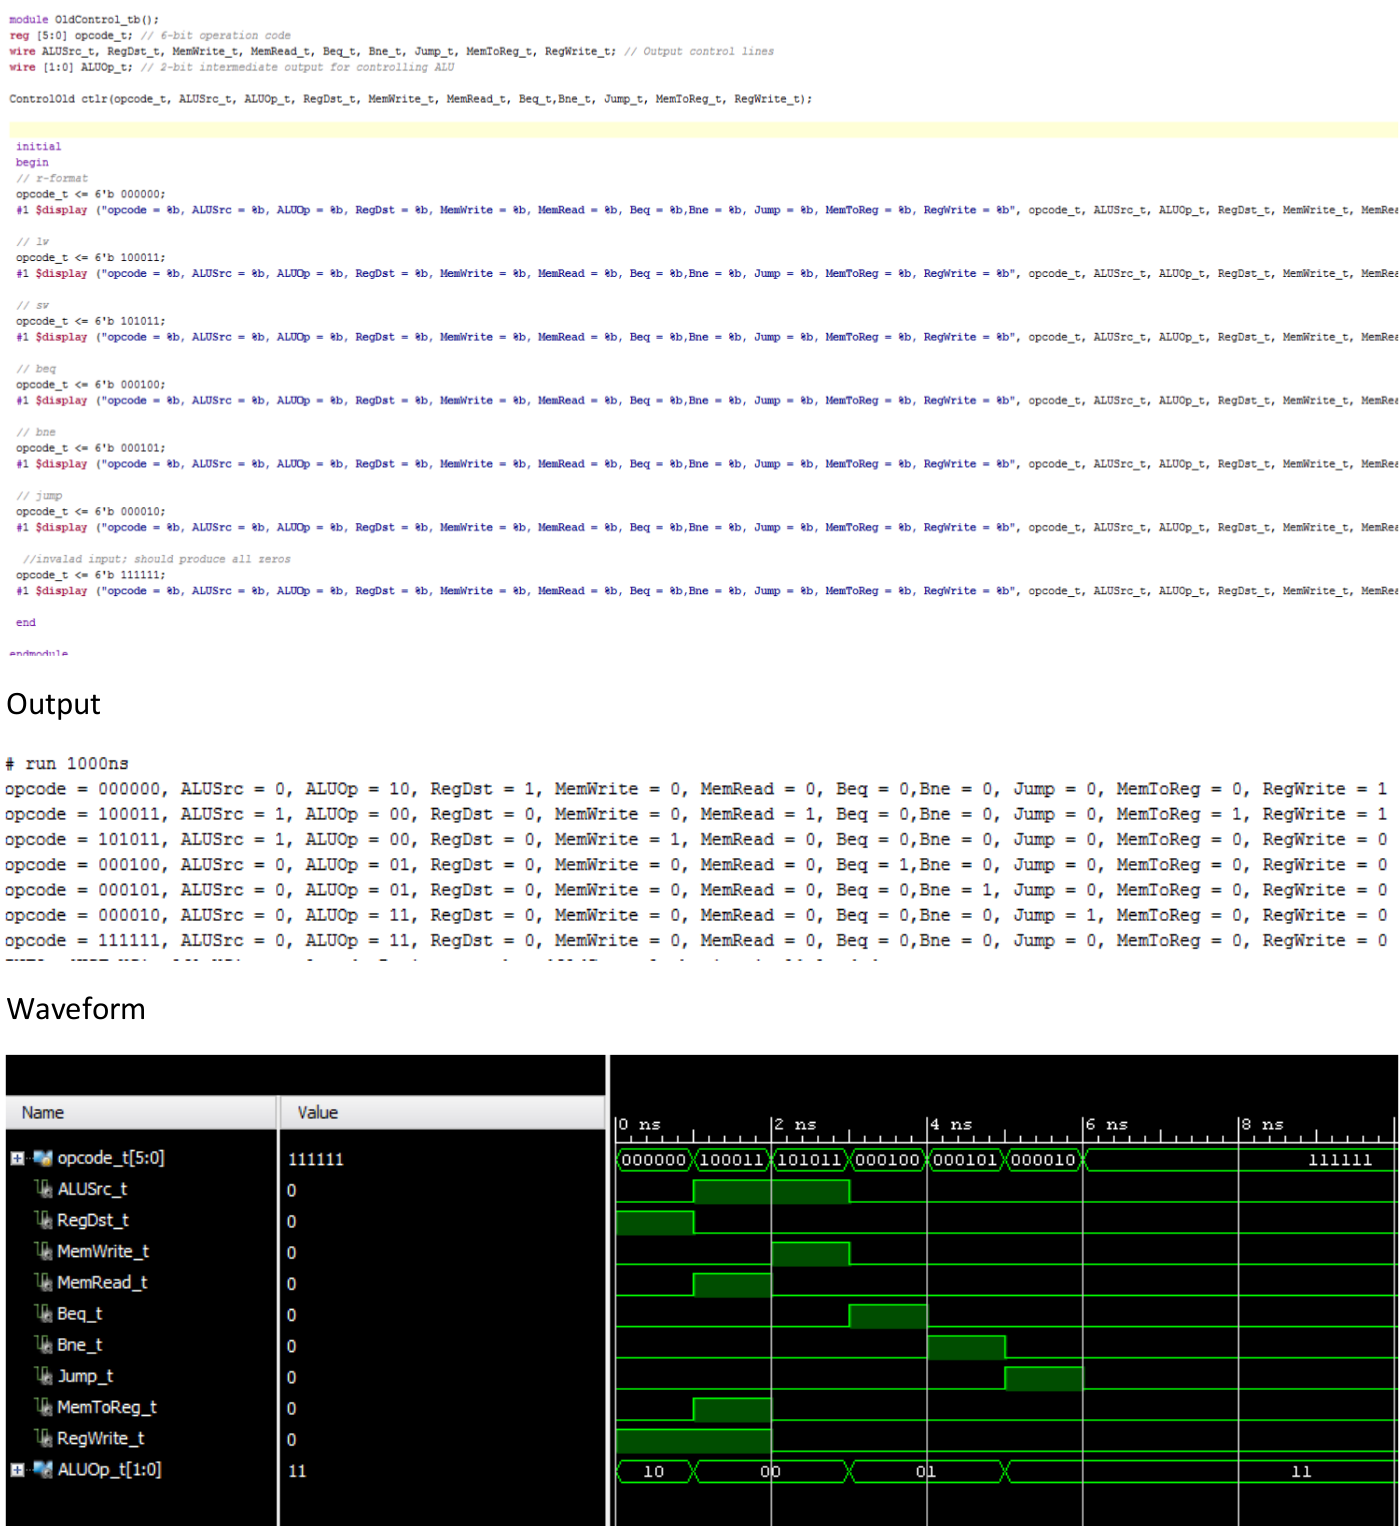
\includegraphics[scale=.3]{images/l.png}
\subsubsection{TB/WF}
\label{co:1}
\includepdf[pages={2}]{../Homework5.pdf}
% same
\subsection{Register File}
\label{alu:1}
\begin{addmargin}[-5em]{-6em}
\lstinputlisting{../registerFile.v}
\end{addmargin}
\subsubsection{TB/WF}
\includepdf[pages={5}]{../Homework5.pdf}
\subsection{ALU Op to Control}
\includepdf[pages={3}]{../Homework5.pdf}
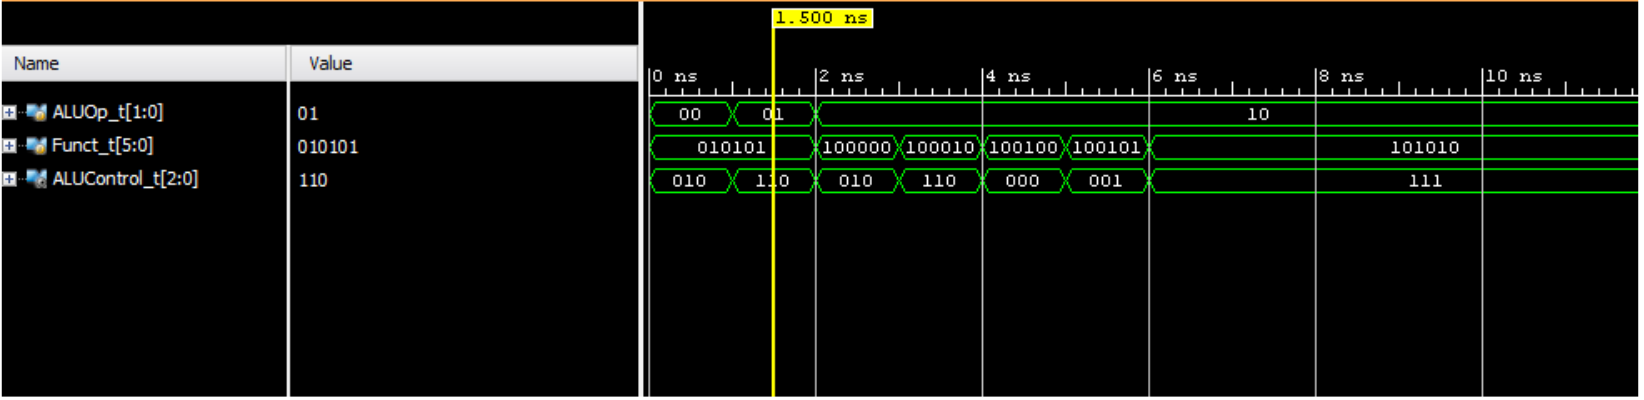
\includegraphics[scale=.2]{images/aluoptoc.png}
\subsection{32 Bit ALU}
\label{alu:1}
\begin{addmargin}[-5em]{-6em}
\lstinputlisting{../ALU32Bit.v}
\end{addmargin}
\subsubsection{ TB/WV}
\begin{addmargin}[-5em]{-6em}
\lstinputlisting{../tests/ALU32_tb.v}
\end{addmargin}
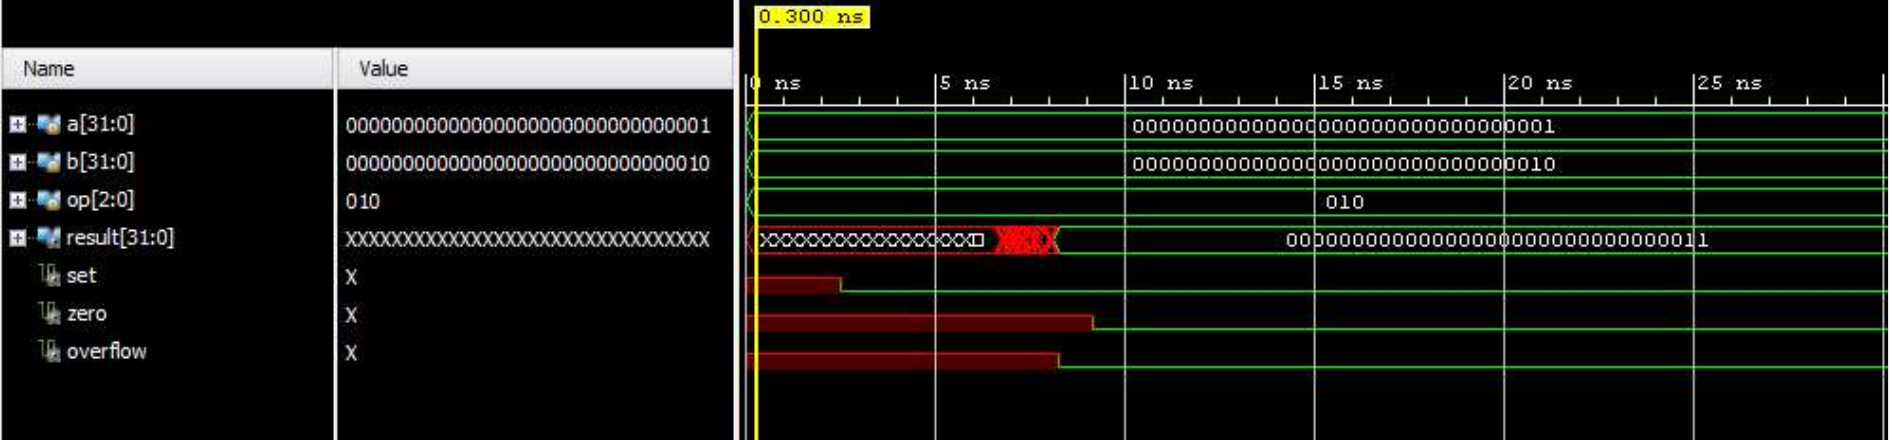
\includegraphics[scale=.2]{images/32BitALU_tb.png}





\subsection{16 Bit ALU}
\label{alu:2}
\begin{addmargin}[-5em]{-6em}
\lstinputlisting{../ALU16.v}
\end{addmargin}
\subsubsection{TB/WF}
\begin{addmargin}[-5em]{-6em}
\lstinputlisting{../tests/ALU16_tb.v}
\end{addmargin}


 %Done no waveform
\subsection{4 Bit ALU}
\label{alu3}
\begin{addmargin}[-5em]{-6em}
\lstinputlisting{../fourbitALU.v}
\end{addmargin}
\subsubsection{TB/WF}
\begin{addmargin}[-5em]{-6em}
\lstinputlisting{../tests/FourBitALU_tb.v}
\end{addmargin}
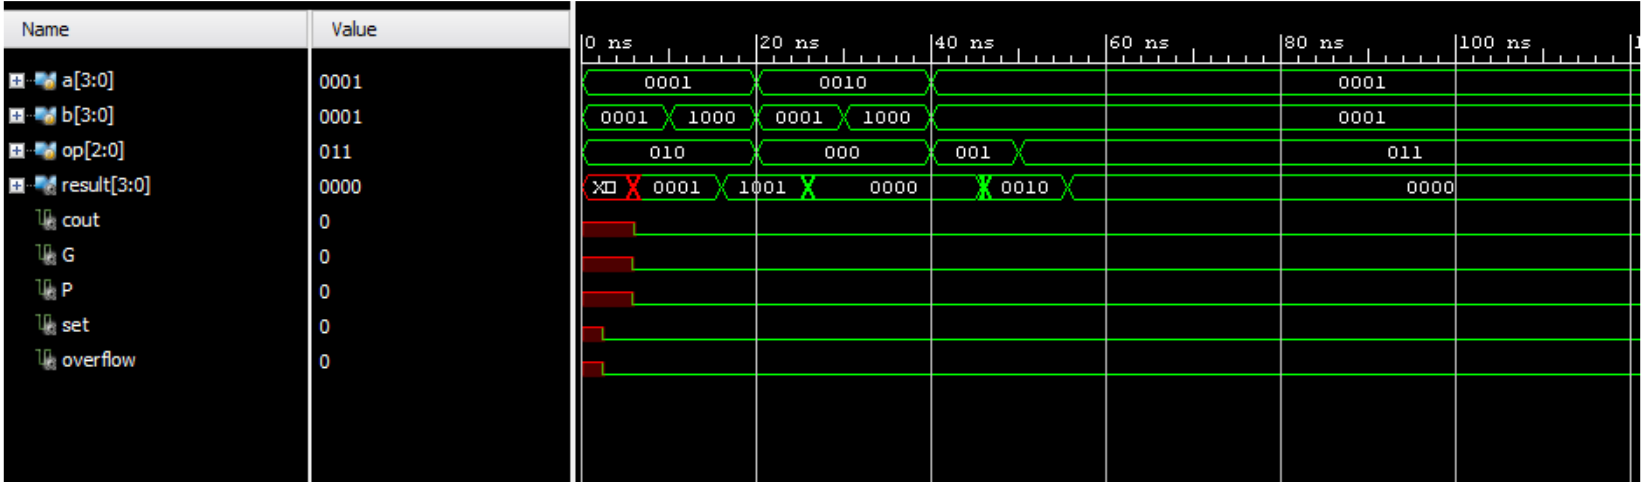
\includegraphics[scale=.2]{images/4bitaluTB.png}


 %Done %Done
\subsection{CLA}
\label{cla:1}
\begin{addmargin}[-5em]{-6em}
  \lstinputlisting{../CLA.v}
\end{addmargin}

\subsubsection{TB/WF}
\begin{addmargin}[-5em]{-6em}
  \lstinputlisting{../tests/CLA_tb.v}
\end{addmargin}
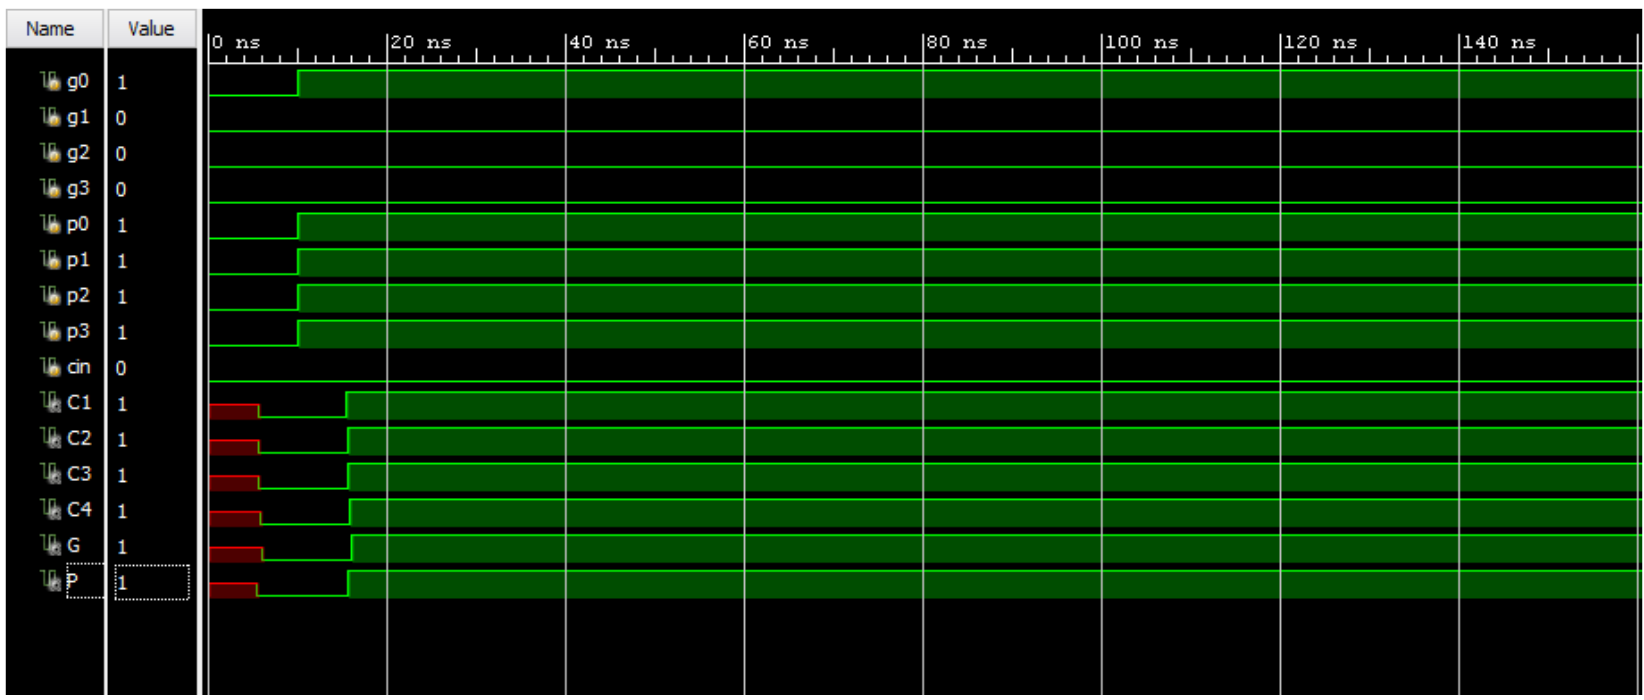
\includegraphics[scale=.2]{images/claWave.png}
%Done
\subsection{1 Bit ALU}
\label{1alu:1}
\begin{addmargin}[-5em]{-6em}
  \lstinputlisting{../onebitALU.v}
\end{addmargin}
\subsubsection{ TB/WF}
\begin{addmargin}[-5em]{-6em}
  \lstinputlisting{../tests/onebitALU_tb.v}
\end{addmargin}
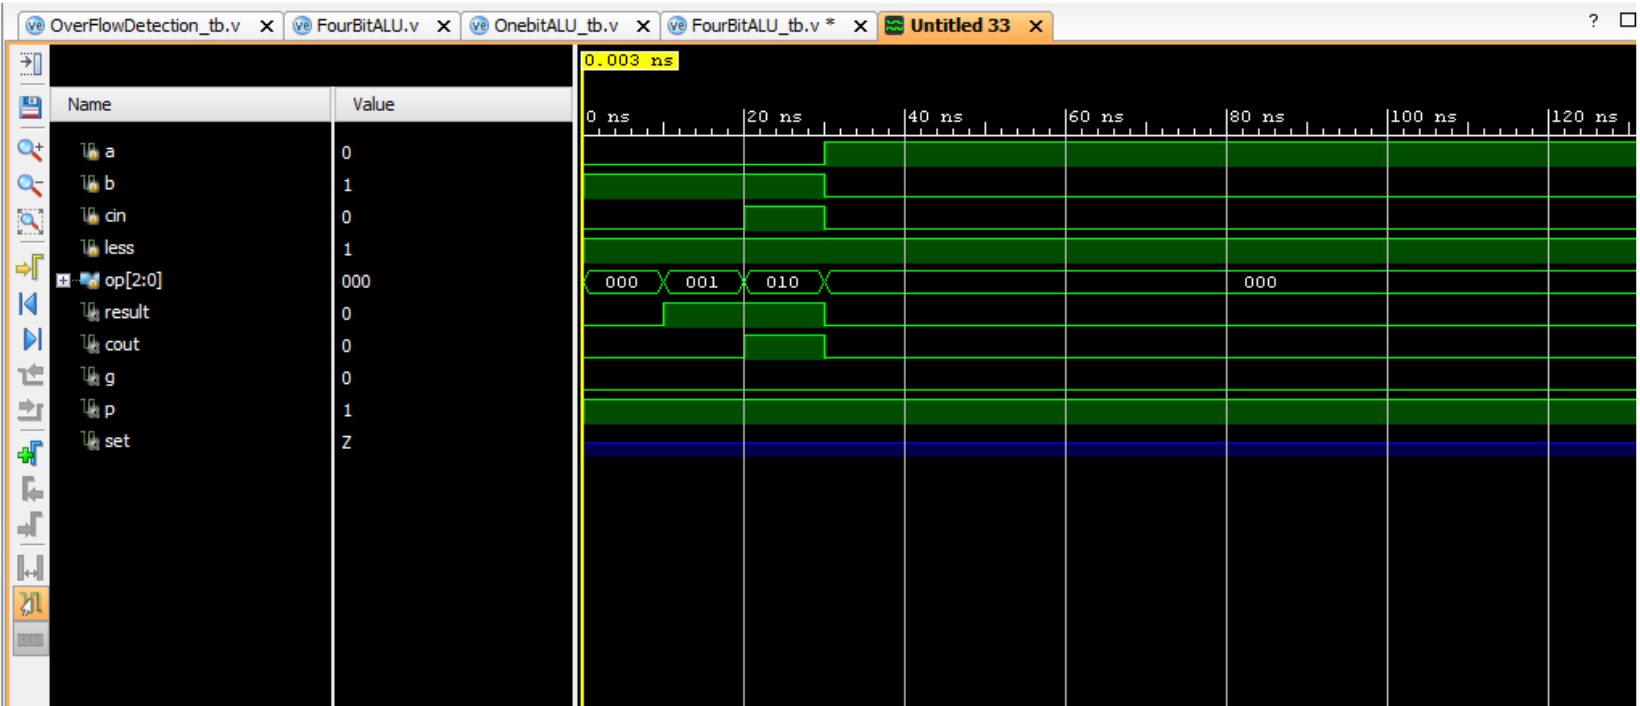
\includegraphics[scale=.2]{images/onebitWave.png} %Done
\subsection{Overflow}
\label{ov:1}
\begin{addmargin}[-5em]{-6em}
\lstinputlisting{../OverFlowDetection.v}
\end{addmargin}
\subsubsection{ TB/WB}

\begin{center}
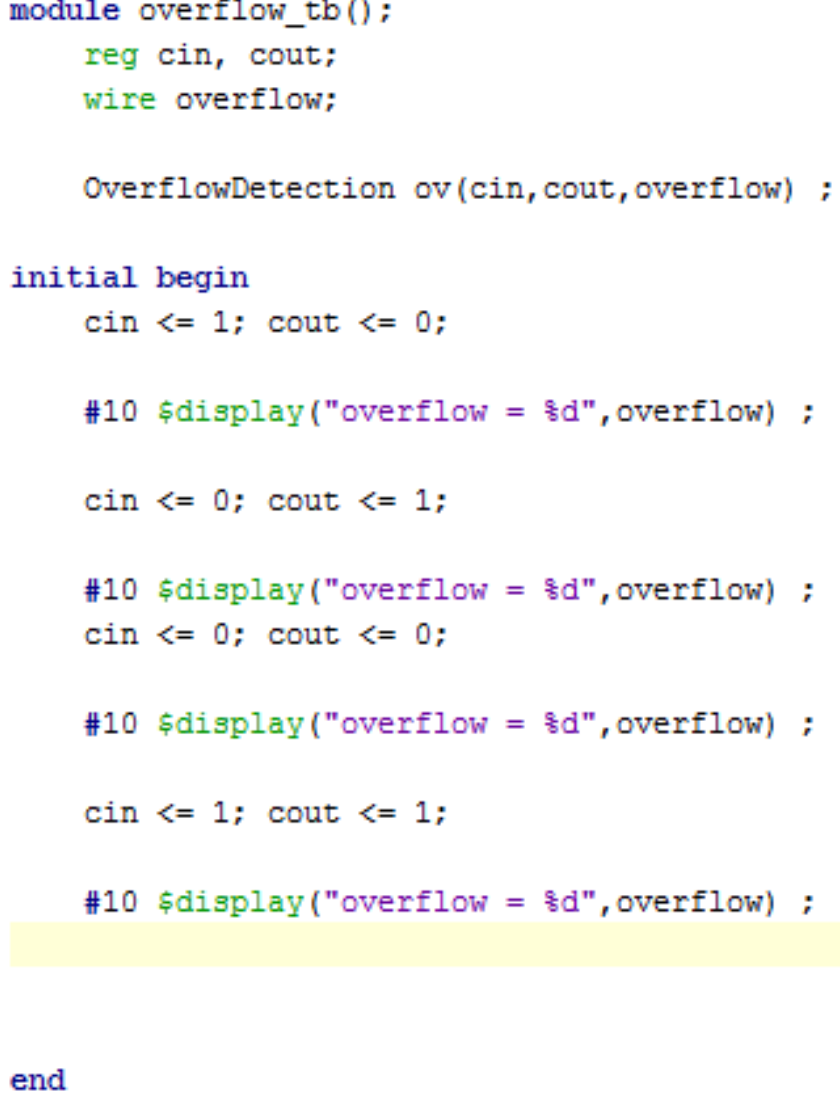
\includegraphics[scale=.2]{images/overflow_tb.png}
\end{center}

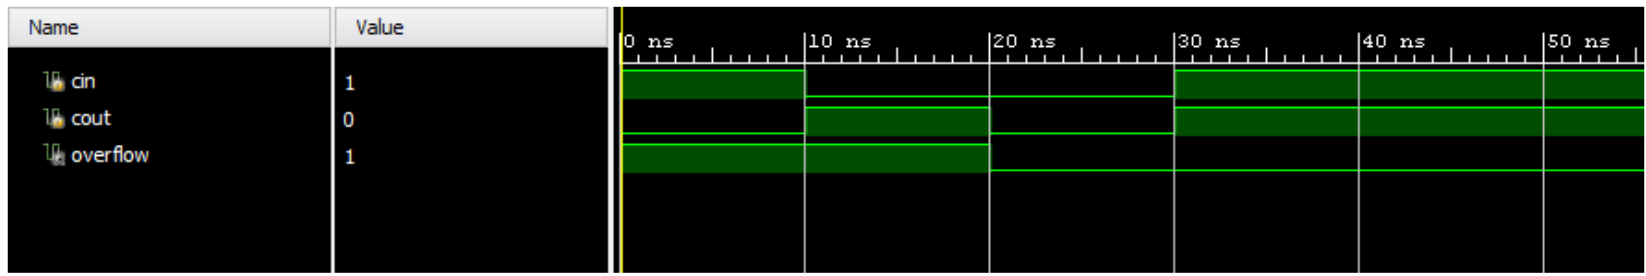
\includegraphics[scale=.2]{images/overflowWave.png}

%% This is inline code \lstinline|Fixpoint f(x : nat) := ...| typeset within a line of text.

%% \paragraph{Para1.} This is a paragraph, or subsubsection.


\cite{*}
\bibliographystyle{plain}
\bibliography{references}


% Done % add description
\subsection{Sign Extension}
\label{se:1}
\begin{addmargin}[-5em]{-6em}
  \lstinputlisting{../SignExtension.v}
\end{addmargin}

\subsubsection{TB/WF}
\begin{addmargin}[-5em]{-6em}
  \lstinputlisting{../tests/SignExtension_tb.v}
\end{addmargin}
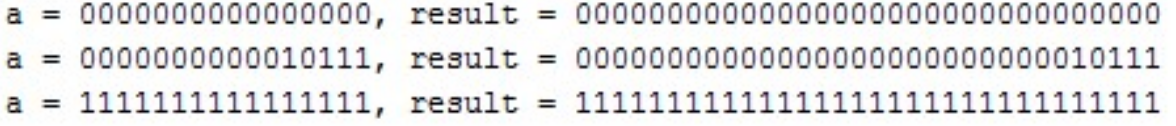
\includegraphics[scale=.2]{images/signExtension.png}


% Add description
 %Add description
\subsection{Mux 32 bit 2 to 1}%Add description
\label{m32:1}
\begin{addmargin}[-5em]{-6em}
  \lstinputlisting{../mux32bit2to1.v}
\end{addmargin}
\subsubsection{TB/WF} 
\begin{addmargin}[-5em]{-6em}
  \lstinputlisting{../tests/mux32_tb.v}
\end{addmargin}
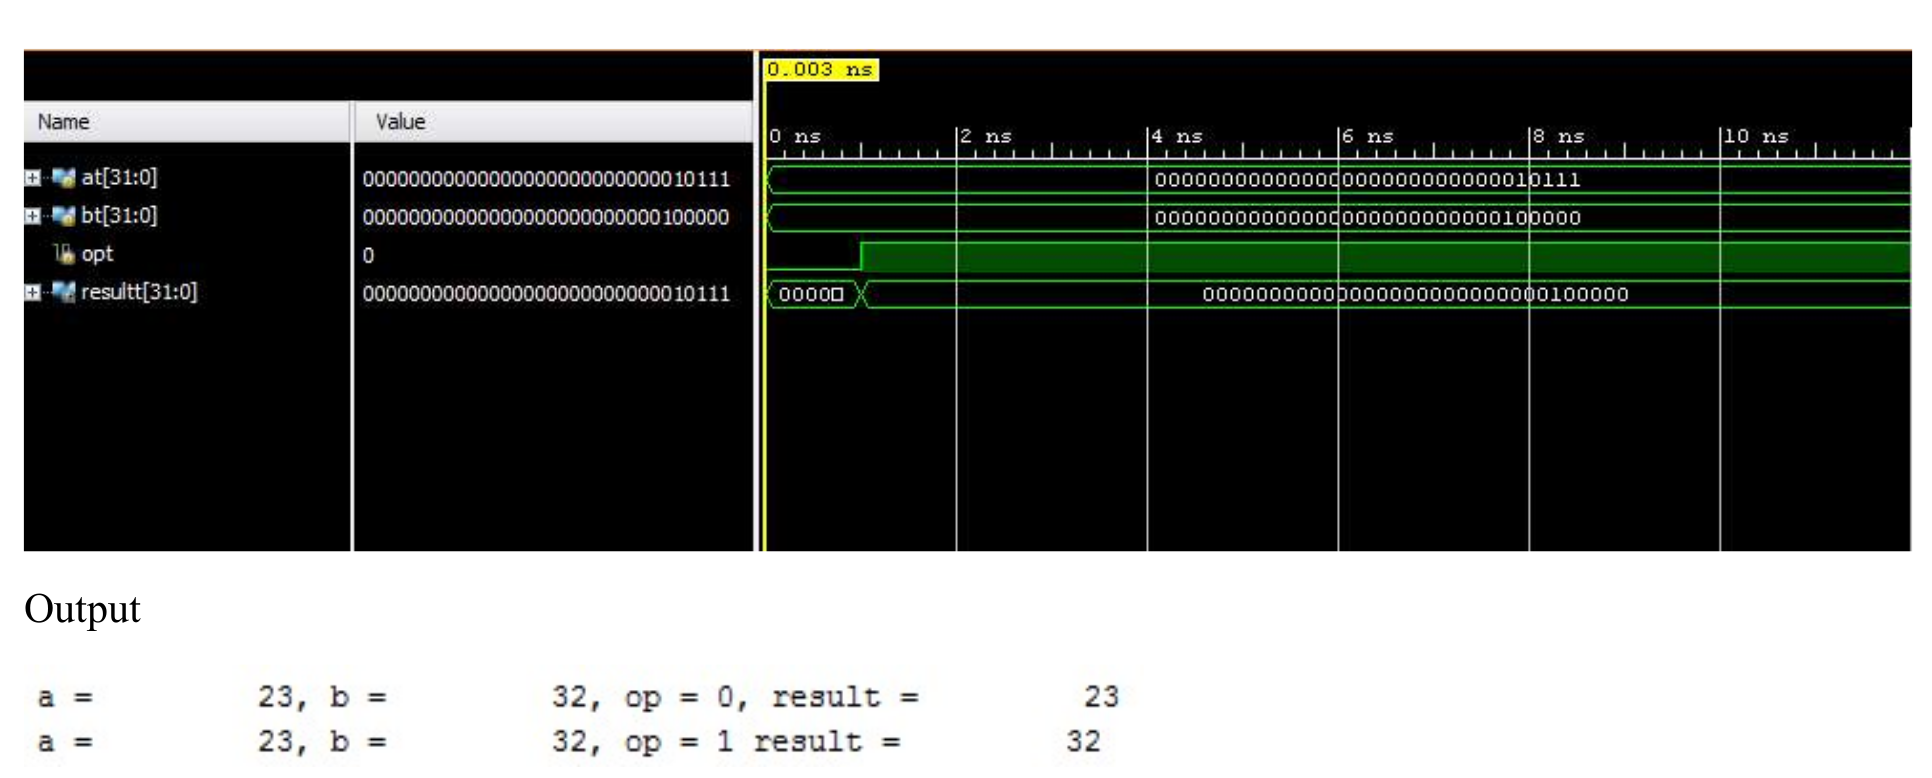
\includegraphics[scale=.2]{images/mux32.png}





\subsection{Mux 5 Bit 2 to 1}
\begin{addmargin}[-5em]{-6em}
  \lstinputlisting{../mux5bit2to1.v}
    \lstinputlisting{../tests/five_tb.v}
\end{addmargin}

\subsection{Forarding}
\label{f:1}
\begin{addmargin}[-5em]{-6em}
  \lstinputlisting{../Forward.v}
\end{addmargin}








\end{document}
